\outclassframe{
\begin{frame}{\ }\relax
    TikZ allows graphics to work according to ``rules''. This is a minus for an arbitrary drawing, but it is an advantage for those drawings that have a given structure and are also built according to ``rules''
\end{frame}
}

{\forcewidefootnote=1
\newcommand{\tikzmark}[1]{\tikz[overlay,remember picture] \node (#1) {};}

\begin{frame}{Graph example 1}\relax
    \twocolImg{
    \only<1>{\inputminted[firstline=9, lastline=10]{latex}{sec01/code/graphSample.tex}
    \inputminted[firstline= 16, lastline=27]{latex}{sec01/code/graphSample.tex}}
    % \only<2>{
    % \smash{\begin{tikzpicture}[overlay, remember picture]
    %         \draw[->, thick] (5.5, -0.5) to[out=0, in=80] +(3.8, 0.3);
    %     \end{tikzpicture}}
    % \inputminted[firstline=26, lastline=26, fontsize=\tt\nornalsize]{latex}{sec01/code/graphSample.tex}
        
    % }
    }{graphSample}
    
     
     \only<1>{You can write \ccol{below=of <label>} to have a relative coordinate}
     
\end{frame}
}

{\forcewidefootnote=1
\begin{frame}{Chain example\magicPage}{}\relax
    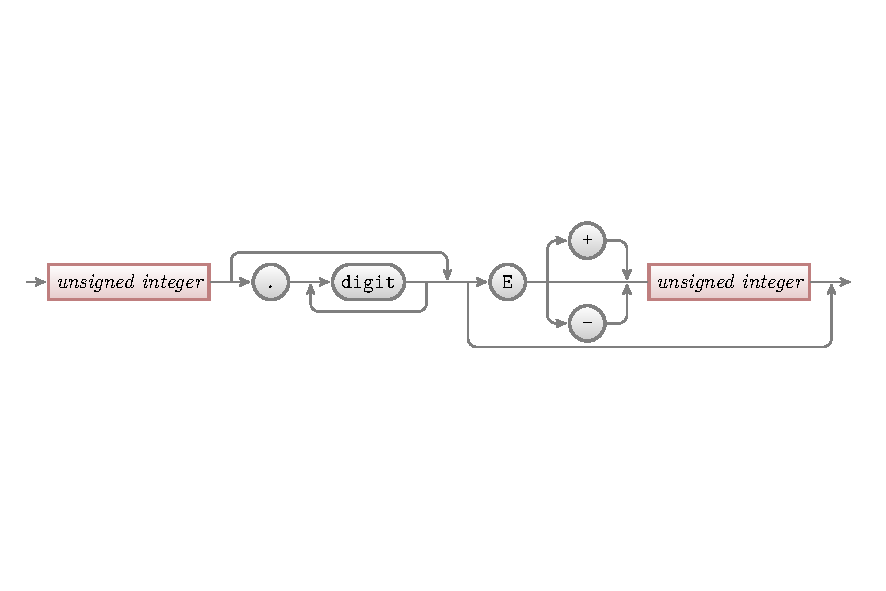
\includegraphics[width=\textwidth]{chainSample}
    
    \vspace{-2em}
    \inputminted[firstline= 9, lastline=10, fontsize=\tt\tiny]{latex}{sec01/code/chainSample.tex}
    \inputminted[firstline= 16, lastline=32, fontsize=\tt\tiny]{latex}{sec01/code/chainSample.tex}

     \skfootnote{\tikzc{I.5}[69]}
\end{frame}
}

\begin{frame}{Tree}

\twocolImg{
\inputminted[firstline=9, lastline=9]{latex}{sec01/code/treeSample.tex}
\inputminted[firstline= 16, lastline=25]{latex}{sec01/code/treeSample.tex}
}{treeSample}

We use \ccol\node\ and \ccol{child}.

\ccol{sibling distance} option provides a horizontal distance between nodes
     
\end{frame}

\inclassframe{
\begin{frame}{\exFrame{reproduce the following with tikZ}}{lvl 1. \textit{You can use absolute coodrinates}}\relax



     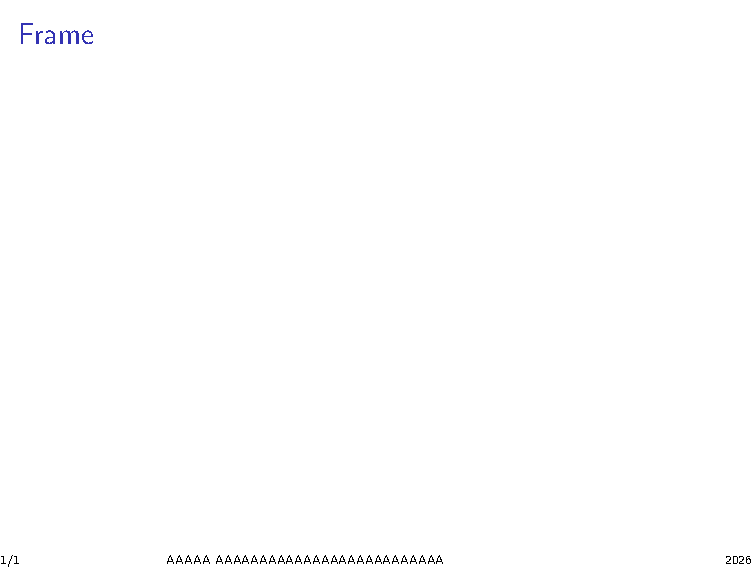
\includegraphics[width=0.4\textwidth]{exLvl1}
\end{frame}

\begin{frame}{\exFrame{reproduce the following with tikZ}}{lvl 2. \textit{You can't use absolute coodrinates}}\relax

     
     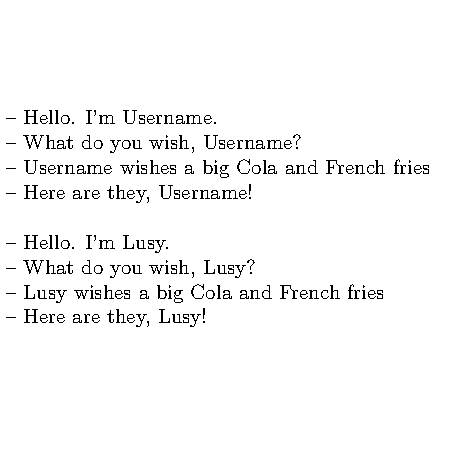
\includegraphics[width=0.4\textwidth]{exLvl2}
\end{frame}

}


